% Part: history
% Chapter: set-theory
% Section: limits

\documentclass[../../../include/open-logic-section]{subfiles}

\begin{document}

\olfileid{his}{set}{limits}	

\olsection{حدّاں دی دقیق تعریف}

اج کل پچھلے مسئلے دا معیاری حل ایہ اے کہ لامتناہی طور اُتے چھوٹیاں قدراں دی لوڑ مکائی جاوے۔ ایہ کم ایویں ہوندا اے۔

اسیں ویکھیا اے کہ جیویں $\beta$ چھوٹا ہوندا اے، ڈھلوان دا اندازہ ہور نیڑے ہوندا اے۔ اصل وچ، جیویں $\beta$، $0$ دے جِنّا مرزی نیڑے جاندا اے، $f'(c)$ دی قدر اوس ڈھلوان ول «بناں روک ودھدی جاندی اے» جیہڑی سانوں چاہیدی اے۔ سو ایہ ویکھن دی تھاں کہ \emph{عین} $\beta = 0$ اُتے کیہ ہوندا اے، سانوں بس $f'(c)$ دا \emph{رُخ} ویکھنا چاہیدا اے، جدوں $\beta$، $0$ ول جاندا اے۔

ایس طرح آکھیے تاں عام مسئلہ ایس شکل دے دعویاں نوں سمجھنا اے:
\begin{center}
جیویں $x$، $c$ دے نیڑے جاندا اے، $g(x)$ بناں روک $\ell$ ول جاندا اے۔
\end{center}
ایہ گل ہور مختصر ایویں لکھ سکدے آں:
\[
\lim_{x \rightarrow c}g(x) = \ell.
\]
انیسویں صدی وچ وائرشٹراس نے کوشی دے پچھلے کم دی بنیاد اُتے ایس عبارت دی پوری طرح دقیق تعریف دتی۔ خیال ایہ اے کہ اسیں $g(x)$ نوں~$\ell$ دے جِنّا چاہو اُنا نیڑے لیا سکدے آں، جے $x$ نوں~$c$ دے مناسب نیڑے لے آئیے۔ ہور ٹھیک ٹھیک آکھیے تاں $\lim_{x \rightarrow c} g(x) = \ell$ دا مطلب ایہ اے:
\[
(\forall\epsilon > 0)(\exists \delta > 0)\forall x \left(|x - c| < \delta \lif |g(x) - \ell| < \epsilon \right).
\]
ایتھے کھڑیاں لکیراں مطلق قدر دسدیاں نیں۔ یعنی $|x| = x$
جدوں $x \geq 0$ ہووے، تے $|x| =-x$ جدوں $x < 0$ ہووے۔ \emph{اوس} فنکشن دا گراف ایویں بنا سکدے او:
\begin{center}
	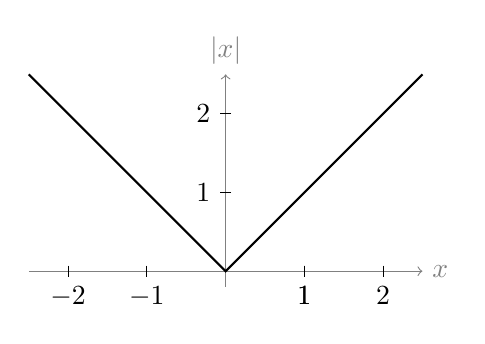
\begin{tikzpicture}[scale=1]
	\draw[->, gray] (-2.5,0) -- (2.5,0) node[right] {$x$};
	\draw[->, gray] (0,-.2) -- (0,2.5) node[above] {$|x|$};
	
	\foreach \x/\xtext in {-2/-2, -1,1, 1/1, 2/2}
	\draw[shift={(\x,0)}] (0pt,2pt) -- (0pt,-2pt) node[below] {{$\xtext$}};
	
	\foreach \y/\ytext in {1/1, 2/2}
	\draw[shift={(0,\y)}] (2pt,0pt) -- (-2pt,0pt) node[left] {{$\ytext$}};
	
	\draw[thick] (-2.5, 2.5)--(0,0)--(2.5, 2.5);
	\end{tikzpicture}
\end{center}
سو تعریف دا موٹا جیہا مطلب ایہ اے کہ تسی اپنی «غلطی» $\epsilon$ توں گھٹ (یعنی $|g(x) - \ell| < \epsilon$) کر سکدے او۔ ایس لئی ایہو جیہیاں مدخلی قدراں چُنو جیہڑیاں $\delta$ توں ودھ دُور~$c$ توں نہ ہون (یعنی $|x -
c| < \delta$)۔

حد دی تعریف ہو جان پچھوں، اسیں لامتناہی طور اُتے چھوٹیاں قدراں نوں پورا ای پاسے رکھ سکدے آں، تے ایہ طے کر سکدے آں کہ $f$ دی $c$ اُتے ڈھلوان ایویں ملدی اے:
\[
	{f}'(c) = \lim_{x \rightarrow 0}\left(\frac{f(c +x) - f(c)}{x}\right) \text{ جتھے حد موجود ہووے}.
\]
ایہ سمجھنا ضروری اے کہ ساڈی تعریف وچ «جتھے حد موجود ہووے» والی شرط کیوں چاہیدی اے۔ اک سوکھی مثال لئی $f(x) = |x|$ لو، جیہدا گراف اسیں ہُنے ویکھیا اے۔ صاف اے کہ $f'(0)$ دی تعریف نہیں بندی۔ جے «سجّے پاسے توں» $0$ ول آئیے، تاں ڈھلوان ہمیشہ $1$ اے۔ جے «کھبّے پاسے توں» $0$ ول آئیے، تاں ڈھلوان ہمیشہ $-1$ اے۔ سو حد دی تعریف نہیں بندی۔ ایس حساب نال اسیں ایہ وی آکھ سکدے آں کہ فنکشن~$f$،~$x$ اُتے اُدوں تے صرف اُدوں \emph{تفریق جوگ} اے جدوں ایہو جیہی حد موجود ہووے۔

اسیں ویکھیا اے کہ \emph{حد} دے خیال نال تفریق کِویں سمجھائی جاندی اے۔ ایہو خیال \emph{مسلسل} فنکشن دی تعریف کرن لئی وی ورت سکدے آں۔ (بولزانو نوں ایہ گل 1817 تک، عملی طور اُتے، سمجھ آ چکی سی۔) کوشی--وائرشٹراس دے طریقے وچ تسلسل نوں ایویں سمجھیا جاندا اے۔ موٹے طور اُتے فنکشن~$f$ (کسے نقطے اُتے) مسلسل اے جے تسی اوہدے حاصل وچ جِنّی درستی منگو، مدخل اُتے درستی دی ڈھکدی شرط لا کے اُنی درستی پکی کیتی جا سکے۔ ہور ٹھیک ٹھیک آکھیے تاں $f$، $c$ اُتے مسلسل اے جے جیویں $x$ صفر ول جاندا اے، $f(c + x)$ تے $f(c)$ دا فرق آپ $0$ ول جاوے۔ دوجے لفظاں وچ $f$، $c$ اُتے اُدوں تے صرف اُدوں \emph{مسلسل} اے جدوں $f(c) = \lim_{x \rightarrow c} f(x)$۔

ہور اگے جائیے تاں گل حقیقی تجزیے ول ٹُر پئے گی، حالانکہ ساڈا موضوع سیٹ نظریہ اے۔ ایس لئی ہُن ایتھے رک کے ایس گل دا نچوڑ دَس دیئے۔ انیسویں صدی وچ ریاضی داناں نے دقیق تعریف والی \emph{حد} ورت کے لامتناہی طور اُتے چھوٹیاں قدراں توں بناں کم کرنا سِکھ لیا۔

\end{document}
